\documentclass[11pt]{article}
\usepackage{latexsym}
\usepackage{amsmath}
\usepackage{amssymb}
\usepackage{amsthm}
\usepackage{epsfig}
\usepackage[tight]{subfigure}

\usepackage{amsmath}

\DeclareMathOperator*{\minimize}{min}
\DeclareMathOperator*{\maximize}{max}

\usepackage{algorithm}
 %on linux you may need to run sudo apt-get install texlive-full to install algorithm.sys
\usepackage{algorithmic}

\usepackage{verbatim}

%%%%%%%%%%%%%%%%%%%%%%%%%%%%%%%%%%%%%%%%%%
% Custom commands                        %
%%%%%%%%%%%%%%%%%%%%%%%%%%%%%%%%%%%%%%%%%%

\newcommand{\vc}[1]{\boldsymbol{#1}}
\newcommand{\adj}[1]{\frac{d J}{d #1}}
\newcommand{\chain}[2]{\adj{#2} = \adj{#1}\frac{d #1}{d #2}}

% mathcal
\newcommand{\Ac}{\mathcal{A}}
\newcommand{\Bc}{\mathcal{B}}
\newcommand{\Cc}{\mathcal{C}}
\newcommand{\Dc}{\mathcal{D}}
\newcommand{\Ec}{\mathcal{E}}
\newcommand{\Fc}{\mathcal{F}}
\newcommand{\Gc}{\mathcal{G}}
\newcommand{\Hc}{\mathcal{H}}
\newcommand{\Ic}{\mathcal{I}}
\newcommand{\Jc}{\mathcal{J}}
\newcommand{\Kc}{\mathcal{K}}
\newcommand{\Lc}{\mathcal{L}}
\newcommand{\Mc}{\mathcal{M}}
\newcommand{\Nc}{\mathcal{N}}
\newcommand{\Oc}{\mathcal{O}}
\newcommand{\Pc}{\mathcal{P}}
\newcommand{\Qc}{\mathcal{Q}}
\newcommand{\Rc}{\mathcal{R}}
\newcommand{\Sc}{\mathcal{S}}
\newcommand{\Tc}{\mathcal{T}}
\newcommand{\Uc}{\mathcal{U}}
\newcommand{\Vc}{\mathcal{V}}
\newcommand{\Wc}{\mathcal{W}}
\newcommand{\Xc}{\mathcal{X}}
\newcommand{\Yc}{\mathcal{Y}}
\newcommand{\Zc}{\mathcal{Z}}

% mathbb
\newcommand{\Ab}{\mathbb{A}}
\newcommand{\Bb}{\mathbb{B}}
\newcommand{\Cb}{\mathbb{C}}
\newcommand{\Db}{\mathbb{D}}
\newcommand{\Eb}{\mathbb{E}}
\newcommand{\Fb}{\mathbb{F}}
\newcommand{\Gb}{\mathbb{G}}
\newcommand{\Hb}{\mathbb{H}}
\newcommand{\Ib}{\mathbb{I}}
\newcommand{\Jb}{\mathbb{J}}
\newcommand{\Kb}{\mathbb{K}}
\newcommand{\Lb}{\mathbb{L}}
\newcommand{\Mb}{\mathbb{M}}
\newcommand{\Nb}{\mathbb{N}}
\newcommand{\Ob}{\mathbb{O}}
\newcommand{\Pb}{\mathbb{P}}
\newcommand{\Qb}{\mathbb{Q}}
\newcommand{\Rb}{\mathbb{R}}
\newcommand{\Sb}{\mathbb{S}}
\newcommand{\Tb}{\mathbb{T}}
\newcommand{\Ub}{\mathbb{U}}
\newcommand{\Vb}{\mathbb{V}}
\newcommand{\Wb}{\mathbb{W}}
\newcommand{\Xb}{\mathbb{X}}
\newcommand{\Yb}{\mathbb{Y}}
\newcommand{\Zb}{\mathbb{Z}}

% mathbf lowercase
\newcommand{\av}{\mathbf{a}}
\newcommand{\bv}{\mathbf{b}}
\newcommand{\cv}{\mathbf{c}}
\newcommand{\dv}{\mathbf{d}}
\newcommand{\ev}{\mathbf{e}}
\newcommand{\fv}{\mathbf{f}}
\newcommand{\gv}{\mathbf{g}}
\newcommand{\hv}{\mathbf{h}}
\newcommand{\iv}{\mathbf{i}}
\newcommand{\jv}{\mathbf{j}}
\newcommand{\kv}{\mathbf{k}}
\newcommand{\lv}{\mathbf{l}}
\newcommand{\mv}{\mathbf{m}}
\newcommand{\nv}{\mathbf{n}}
\newcommand{\ov}{\mathbf{o}}
\newcommand{\pv}{\mathbf{p}}
\newcommand{\qv}{\mathbf{q}}
\newcommand{\rv}{\mathbf{r}}
\newcommand{\sv}{\mathbf{s}}
\newcommand{\tv}{\mathbf{t}}
\newcommand{\uv}{\mathbf{u}}
\newcommand{\vv}{\mathbf{v}}
\newcommand{\wv}{\mathbf{w}}
\newcommand{\xv}{\mathbf{x}}
\newcommand{\yv}{\mathbf{y}}
\newcommand{\zv}{\mathbf{z}}

% mathbf uppercase
\newcommand{\Av}{\mathbf{A}}
\newcommand{\Bv}{\mathbf{B}}
\newcommand{\Cv}{\mathbf{C}}
\newcommand{\Dv}{\mathbf{D}}
\newcommand{\Ev}{\mathbf{E}}
\newcommand{\Fv}{\mathbf{F}}
\newcommand{\Gv}{\mathbf{G}}
\newcommand{\Hv}{\mathbf{H}}
\newcommand{\Iv}{\mathbf{I}}
\newcommand{\Jv}{\mathbf{J}}
\newcommand{\Kv}{\mathbf{K}}
\newcommand{\Lv}{\mathbf{L}}
\newcommand{\Mv}{\mathbf{M}}
\newcommand{\Nv}{\mathbf{N}}
\newcommand{\Ov}{\mathbf{O}}
\newcommand{\Pv}{\mathbf{P}}
\newcommand{\Qv}{\mathbf{Q}}
\newcommand{\Rv}{\mathbf{R}}
\newcommand{\Sv}{\mathbf{S}}
\newcommand{\Tv}{\mathbf{T}}
\newcommand{\Uv}{\mathbf{U}}
\newcommand{\Vv}{\mathbf{V}}
\newcommand{\Wv}{\mathbf{W}}
\newcommand{\Xv}{\mathbf{X}}
\newcommand{\Yv}{\mathbf{Y}}
\newcommand{\Zv}{\mathbf{Z}}

% bold greek lowercase
\newcommand{\alphav     }{\boldsymbol \alpha     }
\newcommand{\betav      }{\boldsymbol \beta      }
\newcommand{\gammav     }{\boldsymbol \gamma     }
\newcommand{\deltav     }{\boldsymbol \delta     }
\newcommand{\epsilonv   }{\boldsymbol \epsilon   }
\newcommand{\varepsilonv}{\boldsymbol \varepsilon}
\newcommand{\zetav      }{\boldsymbol \zeta      }
\newcommand{\etav       }{\boldsymbol \eta       }
\newcommand{\thetav     }{\boldsymbol \theta     }
\newcommand{\varthetav  }{\boldsymbol \vartheta  }
\newcommand{\iotav      }{\boldsymbol \iota      }
\newcommand{\kappav     }{\boldsymbol \kappa     }
\newcommand{\varkappav  }{\boldsymbol \varkappa  }
\newcommand{\lambdav    }{\boldsymbol \lambda    }
\newcommand{\muv        }{\boldsymbol \mu        }
\newcommand{\nuv        }{\boldsymbol \nu        }
\newcommand{\xiv        }{\boldsymbol \xi        }
\newcommand{\omicronv   }{\boldsymbol \omicron   }
\newcommand{\piv        }{\boldsymbol \pi        }
\newcommand{\varpiv     }{\boldsymbol \varpi     }
\newcommand{\rhov       }{\boldsymbol \rho       }
\newcommand{\varrhov    }{\boldsymbol \varrho    }
\newcommand{\sigmav     }{\boldsymbol \sigma     }
\newcommand{\varsigmav  }{\boldsymbol \varsigma  }
\newcommand{\tauv       }{\boldsymbol \tau       }
\newcommand{\upsilonv   }{\boldsymbol \upsilon   }
\newcommand{\phiv       }{\boldsymbol \phi       }
\newcommand{\varphiv    }{\boldsymbol \varphi    }
\newcommand{\chiv       }{\boldsymbol \chi       }
\newcommand{\psiv       }{\boldsymbol \psi       }
\newcommand{\omegav     }{\boldsymbol \omega     }

% bold greek uppercase
\newcommand{\Gammav     }{\boldsymbol \Gamma     }
\newcommand{\Deltav     }{\boldsymbol \Delta     }
\newcommand{\Thetav     }{\boldsymbol \Theta     }
\newcommand{\Lambdav    }{\boldsymbol \Lambda    }
\newcommand{\Xiv        }{\boldsymbol \Xi        }
\newcommand{\Piv        }{\boldsymbol \Pi        }
\newcommand{\Sigmav     }{\boldsymbol \Sigma     }
\newcommand{\Upsilonv   }{\boldsymbol \Upsilon   }
\newcommand{\Phiv       }{\boldsymbol \Phi       }
\newcommand{\Psiv       }{\boldsymbol \Psi       }
\newcommand{\Omegav     }{\boldsymbol \Omega     }


\newcommand{\handout}[5]{
  \noindent
  \begin{center}
  \framebox{
    \vbox{
      \hbox to 5.78in { {#1} \hfill #2 }
      \vspace{4mm}
      \hbox to 5.78in { {\Large \hfill #5  \hfill} }
      \vspace{2mm}
      \hbox to 5.78in { {\em #3 \hfill #4} }
    }
  }
  \end{center}
  \vspace*{4mm}
}

\newcommand{\lecture}[5]{\handout{#1}{#2}{#3}{#4}{#5}}
\newcommand{\collision}[0]{\mathrm{collision}}
\newcommand{\nocollision}[0]{\overline{\collision}}

\newcommand*{\QED}{\hfill\ensuremath{\square}}

\newtheorem{theorem}{Theorem}
\newtheorem{corollary}[theorem]{Corollary}
\newtheorem{lemma}[theorem]{Lemma}
\newtheorem{observation}[theorem]{Observation}
\newtheorem{proposition}[theorem]{Proposition}
\newtheorem{definition}[theorem]{Definition}
\newtheorem{claim}[theorem]{Claim}
\newtheorem{fact}[theorem]{Fact}
\newtheorem{assumption}[theorem]{Assumption}
\newtheorem{note}[theorem]{Note}

% 1-inch margins, from fullpage.sty by H.Partl, Version 2, Dec. 15, 1988.
\topmargin 0pt
\advance \topmargin by -\headheight
\advance \topmargin by -\headsep
\textheight 8.9in
\oddsidemargin 0pt
\evensidemargin \oddsidemargin
\marginparwidth 0.5in
\textwidth 6.5in

\parindent 0in
\parskip 1.5ex
%\renewcommand{\baselinestretch}{1.25}

\begin{document}

\lecture{Statistical Techniques in Robotics (16-831, S21)}{Lecture \#11
  (Wednesday, March 10)}{Lecturer: Kris Kitani}{Scribes: Abhinav Agarwalla, Kshitij Goel}{AdaBoost, Bandits (Explore-Exploit)}

\section{Review}
In the previous lecture, we learnt one algorithm for online supervised learning called Online
Support Vector Machine (Online SVM). We review two variants of this algorithm in this section
(Hard- and Soft-SVM).

\subsection{Max-Margin Classifier}
\begin{figure}[H]
    \centering
    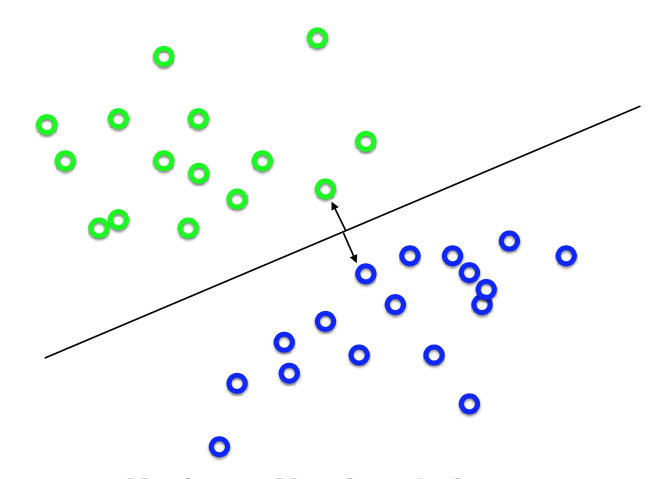
\includegraphics[width=0.5\textwidth]{images/max_margin.png}%
    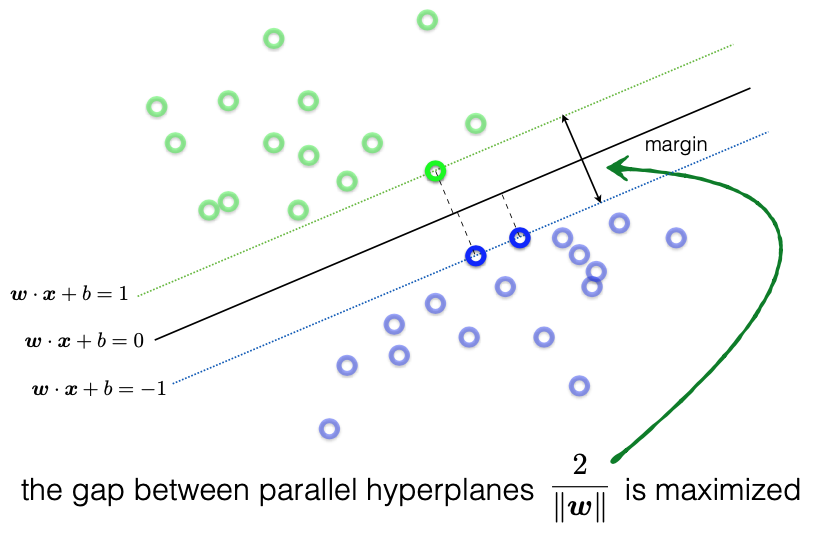
\includegraphics[width=0.5\textwidth]{images/max_margin_2.png}
    \caption{Max-margin classification task is to find a hyperplane that separates the closest
    points in two classes by the maximum amount of distance. Such classification is robust to
    minor perturbations in data.}
    \label{fig:max-margin}
\end{figure}
The max-margin classification task (\ref{fig:max-margin}) aims at finding
a hyperplane that satisfies the objective:
$$\min_{\boldsymbol{w}} \| \boldsymbol{w} \|^2 \quad \text{such that, } y_i (\boldsymbol{w} \cdot \boldsymbol{x}_i + b) \geq 1 \ \forall i = \{ 1, \ldots, N \}$$

However, this formulation assumes that the labeled data is linearly separable, which is a
strong assumption for real-world data (``Hard-SVM"). This assumption is relaxed in the Soft-SVM.

\subsection{Soft-SVM}
Soft-SVM is more robust to noisy boundaries (for example, imagine in
Fig. \ref{fig:max-margin}, if a blue label is on the other side of the margin the Hard-SVM will
not provide a suitable solution). The objective for Soft-SVM introduces slack variable $\xi_i$
for sample $i$ and accounts for miss-classifications:
$$\min_{\boldsymbol{w}, \xi} \| \boldsymbol{w} \|^2 + C \sum_i \xi_i \quad \text{such that, } y_i (\boldsymbol{w} \cdot \boldsymbol{x}_i + b) \geq 1 - \xi_i \ \forall i = \{ 1, \ldots, N \}$$

Here, $C$ is a regularization parameter. When $C$ is small, we ignore the constraints more and
hence the margin of the resulting solution is large. As $C \rightarrow \infty$, Soft-SVM tends
to Hard-SVM.

\subsection{Hinge Loss and Sub-Gradients}
To solve the Soft-SVM, we rewrite the objective as:
$$\min_{\boldsymbol{w}} \frac{\lambda}{2} \| \boldsymbol{w} \|^2 + \frac{1}{M} \sum_{m=1}^M 1 - y_m \boldsymbol{w}^{\top} \boldsymbol{x}_m$$
Notice that the second term is not lower-bounded, it can be a very large negative value for some
correctly classified (easy) points. So, we introduce hinge loss to only consider slightly correct,
slightly mistaken, or very mistaken classifications:
$$\min_{\boldsymbol{w}} \frac{\lambda}{2} \| \boldsymbol{w} \|^2 + \frac{1}{M} \sum_{m=1}^M \max \{0, 1 - y_m \boldsymbol{w}^{\top} \boldsymbol{x}_m \}$$
But the problem with hinge loss is that it is not differentiable, so we cannot take the gradient
in the usual way and use our online mirror descent machinery to find optimal weights. We instead
use sub-gradients (Online Sub-Gradient Descent). There can be many sub-gradients for a convex
function (``differential set"). One of the sub-gradients for the hinge loss is:
\begin{gather*}
    \boldsymbol{z}_m = 
    \begin{cases}
        \mathbf{0} \quad \text{if } y_m \boldsymbol{w}^{\top} \boldsymbol{x}_m \geq 1\\
        -y_m \boldsymbol{x}_m \quad \text{otherwise}
    \end{cases}
\end{gather*}


Overall, SVM similar to perceptrons we saw earlier but with the addition of margin.

\begin{minipage}{0.49\textwidth}
\begin{algorithm}[H]
\caption{Soft-SVM}
\label{algo:soft-svm}
\begin{algorithmic}[1]
\STATE $\boldsymbol{\theta}^{(1)} \leftarrow \mathbf{0} \in \mathbb{R}^N$
\FOR{$t=1,\;\cdots,\;T$}
\STATE $y_d, \boldsymbol{x}_d \sim \boldsymbol{D}$
\STATE $\boldsymbol{\theta}^{(t)} = \boldsymbol{\theta}^{(t-1)} + y_d \boldsymbol{x}_d \cdot \mathbf{1} [y_d (\boldsymbol{w}^{(t)} \cdot \boldsymbol{x}_d) < 1]$
\STATE $\boldsymbol{w}^{(t+1)} \leftarrow \frac{1}{\lambda(t+1)} \boldsymbol{\theta}^{(t)}$
\ENDFOR
\STATE $\bar{\boldsymbol{w}} = \frac{1}{T} \sum_t \boldsymbol{w}^t$
\end{algorithmic}
\end{algorithm}
\end{minipage}
\hfill
\begin{minipage}{0.49\textwidth}
\begin{algorithm}[H]
\caption{Perceptron}
\label{algo:perceptron}
\begin{algorithmic}[1]
\STATE $\textbf{w}^{(1)} \leftarrow \mathbf{0} \in \mathbb{R}^N$
\FOR{$t=1,\;\cdots,\;T$}
\STATE \textsc{Receive} ($\boldsymbol{x}^{(t)}, y^{(t)}$)
\STATE $\boldsymbol{\theta}^{(t)} = \boldsymbol{\theta}^{(t)} + y^{(t)} \boldsymbol{x}^{(t)} \cdot \mathbf{1} [y^{(t)} (\boldsymbol{w}^{(t)} \cdot \boldsymbol{x}_d) < 0]$
\STATE $\boldsymbol{w}^{(t+1)} = \boldsymbol{\theta}^{(t)}$
\ENDFOR
\end{algorithmic}
\end{algorithm}
\end{minipage}

%This section serves as a review of the previous lecture and any other context required to frame the content of the current lecture. 

%You may format the scribes in any way you like, aside from changing font style, size and page format. Please use subsections and paragraphs to increase the readability of your notes.

%Length requirement 1-2 pages.

\section{Summary}
Finding the solution to the Soft-SVM objective was based on using online sub-gradient descent. Now we study
the AdaBoost algorithm which uses randomized weighted majority for its solution.

Before we get into describing the algorithm in detail, we have to define a theoretical framework to judge
a \textit{weak} versus a \textit{strong} learning algorithm. This framework is called the Probably
Approximately Correct (PAC) learning model introduced in \cite{valiant1984theory}.

\subsection{PAC Learning Model}
The PAC learning model is a theoretical framework to answer two questions:
\begin{enumerate}
    \item What is the optimal dataset size to obtain good generalization?
    \item What is the computational cost of learning?
\end{enumerate}

Consider an unknown distribution $P(x, y)$ from which a dataset $\mathcal{D}$ of size $N$ is
drawn (i.e. the class labels are determined by some unknown deterministic distribution
$y = f^* (x)$). The dataset $\mathcal{D}$ can be viewed as an approximation of the original
distribution $P(x, y)$. Now, let $\mathcal{F}$ denote the space of functions and
$\mathcal{F} \mid \mathcal{D}$ denote the subset of $\mathcal{F}$ containing the functions
defined on the basis of the dataset $\mathcal{D}$. Then, a function $f(x ; \mathcal{D})$ drawn
from $\mathcal{F} \mid \mathcal{D}$ can be considered a classifier learned on the dataset
$\mathcal{D}$ and thus an approximation to the deterministic labeling function $f^* (x)$.

\definition{\normalfont \textbf{Generalization}  The function $f(x)$ is said to have a good generalization if the expected error rate is below a pre-defined threshold $\epsilon$, i.e., $$\mathbb{E}_{P(x, y)}[\mathbf{1}[f(x; \mathcal{D}) \neq y]] < \epsilon.$$}
\definition{\normalfont\textbf{PAC Learning Algorithm} A learning algorithm that requires
\textbf{Definition 1} to hold with a pre-defined probability $1 - \delta$ for any dataset
$\mathcal{D}$ drawn from $P(x, y)$.}
\definition{\normalfont\textbf{Strong PAC Learner} A PAC learning algorithm whose output
$f(x)$ produces an error of at most $\epsilon$ with a probability $1-\delta$.}
\definition{\normalfont\textbf{Weak PAC Learner} A PAC learning algorithm whose output
$f(x)$ produces an error of at most $\epsilon \geq 1/2 - \gamma$ with a probability $1-\delta$,
for some $\gamma > 0$.}

\normalfont
At a high-level, the weak PAC learner is flexible in terms of the maximum error while its strong
counterpart is not and requires a maximum error of $\epsilon$. Further, there is a well-known result that
relates the two types of learners via boosting, as shown in \cite{schapire1990strength}.

\subsection{AdaBoost}
The theorem based on \cite{schapire1990strength} suggests that a weak PAC learner can be called
multiple times to generate a sequence of hypothesis with a different subset of $\Dv$ which
can be combined to form a single strong PAC learner. This process is called \textit{boosting}.

Adaboost~\cite{freund1997decision} is a specific learning algorithm in the class of boosting algorithms. In previous online learning methods, one receives new data points at every time instant. In Adaboost, we receive \textit{weak learners} instead of data points. The final prediction rule is a weighted sum of learner predictions upto the current time $T$. Since we have $T$ weak learner at time step $T$, we just use the 'number of weak learners' terminology over time steps.

We study the prediction and update step for Adaboost in the next section. The Adaboost algorithm is detailed in Algorithm \ref{algo:adaboost}. 

\subsubsection{Prediction Step}
Adaboost assumes access to a fixed dataset $\Dv$, over which it defines sample-based weights $\wv$. $\wv^{t}_i$ denotes the weight for $i^{th}$ sample \ie $\xv_i$ and $t^{th}$ learner $h^{(t)}$. It's important to not that weights $\wv$ are now indexed over samples rather than features/experts. The sample weights $\wv^{(0)}$ are initialised uniformly. At each prediction step, a weak learners learn a classifier based on a weights loss using normalised sample weights.

\subsubsection{Update Step}
At each update step, the mean error $\epsilon^{(t)}$ associated with the learned hypothesis $h^{(t)}$ is computed. The error computed is again a weighted accuracy, weighed by the sample weights. Using $\epsilon^{(t)}$ and penalty parameter $\beta^{(t)}$, the weights $\wv^t$ are updated for next learner. For a good classifier $\beta^{(t)} \rightarrow 0$, while for a bad classifier $\beta^{(t)} \rightarrow \infty$.

Interestingly, the update equation for Adaboost is exponential. This comes from the observation that weights $\wv$ are normalised to act like a probability over samples and enforces \textit{entropic regularisation} over the weights. We know that Online Mirror Descent for a linear  objective function and entropic regularisation has an exponential update equation.

Now, let's see if the updates make sense. If the weak leaner $h^{(t)}$ classifies a data point correctly \ie $|h^{(t)}(\xv_n^{(t)}) - y_n^{(t)}| \rightarrow 0$, $\beta^{1-|h^{(t)}(\xv_n^{(t)}) - y_n^{(t)}|} \sim \beta$. If it doesn't, the update is $\sim \beta^2$. In other words, the weights for mis-classified samples are increased while decreased for correctly sampled. This makes sense, since the next weak learner $h^{(t+1)}$ would have a higher penalty on misclassifying the incorrect samples. 

Once all the weaker learner hypothesis' are learned, the final prediction is weighted average of all weak learner. The weights is inversely proportional to the error of weak learners, with higher weights for a learner that makes fewer mistakes.

The error bound for the final hypothesis $\epsilon \le 2^T\prod_{t=1}^{T} \sqrt{\epsilon_t(1 - \epsilon_t)}$. %(Proof in appendix?)
\begin{algorithm}[H]
\caption{Adaboost}
\label{algo:adaboost}
\begin{algorithmic}[1]
\STATE Input: Dataset $\Dv =\{\xv_n, y_n\}_{n=1}^{N}$, where feature vector $\xv_n \in \mathbb{R}^M$ and label $y \in \{0, 1\}$
\STATE Input: Weight vector $\{w^{(0)}\}_{n=1}^{N}$ initialised uniformly
\STATE Input: Number of weak learners $T$ 
\FOR{$t=1,\;\cdots,\;T$}
\STATE $\pv^{(t)} = \wv^{(t-1)}/(\sum_n w_n^{(t-1)})$ 
\STATE $h^{(t)} = \mathtt{WEAKLEARNER}(\Dv, \pv^{(t)})$  \hfill $\triangleright$ Prediction Step
\STATE $\epsilon^{(t)} = \sum_n p^t_n |h^{(t)}(\xv_n) - y_n|$
\STATE $\beta^{(t)} = \frac{\epsilon^{(t)}}{1-\epsilon^{(t)}}$
\STATE $w_n^{(t)} = w_n^{(t-1)}\beta^{1-|h^{(t)}(\xv_n^{(t)}-y_n^{(t)}|} \qquad \forall n$ \hfill $\triangleright$ Weight Update Step
\ENDFOR
\STATE $h_F(\xv) = \mathbbm{1}\left[\sum_{t=1}^T (log(\frac{1}{\beta^{(t)}}))h^{(t)}(\xv) \ge \frac{1}{2} \sum_{t=1}^{T} log(\frac{1}{\beta^{(t)}})\right]$
\end{algorithmic}
\end{algorithm}

\subsubsection{Adaboost and Weighted Majority Algorithm}

\textbf{Differences}. The major difference between Adaboost and WMA is that Adaboost weights samples instead of experts or features as done by Weighted Majority Agorithm (WMA). Adaboost learns a new weak hypothesis at each prediction step, while WMA just selects a hypothesis/expert randomly.

\textbf{Similarities}: Both utilise entropic regularisation over weights, and hence have exponential updates.

\subsection{Multi-Armed Bandit}
We now shift from online supervised learning to studying Multi-Armed Bandit (MAB) problem.
\begin{figure}[H]
    \centering
    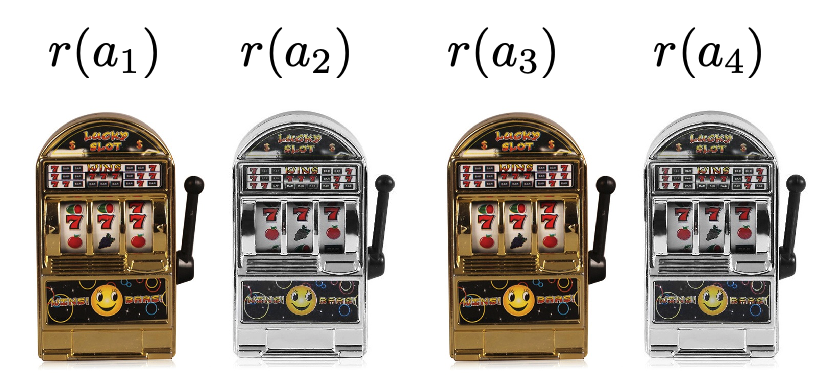
\includegraphics[width=0.5\textwidth]{images/bandit_intro.png}%
    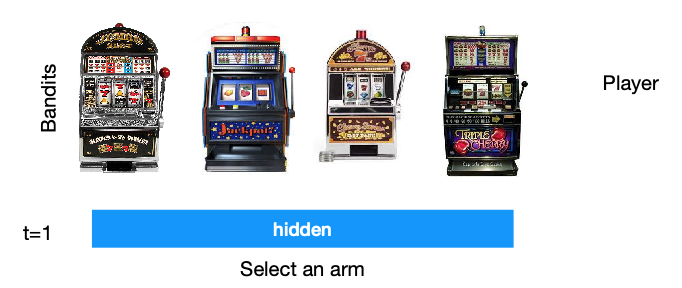
\includegraphics[width=0.5\textwidth]{images/bandit_pwea.png}
    \caption{Introduction to the Multi-Armed Bandit (MAB) problem. (Left) The problem assumes
    an unknown reward distribution behind multiple slot machines (``bandits"). (Right) When
    a player pulls an arm and gets an output (``reward"), it is not shown the outputs (``rewards") of other arms
    (partial observability).
    This is in contrast to the Prediction with Expert Advice (PWEA) scenario where the player
    knows the outputs of all the experts (full observability).}
    \label{fig:bandit}
\end{figure}

Figure \ref{fig:bandit} illustrates the multi-armed bandit problem. A few observations about the
feedback in this learning problem:
\begin{enumerate}
    \item \textbf{One-Shot Feedback}: This is because one action from the player leads to one
    reward and selecting any particular action does not change the state at the next time-step.
    \item \textbf{Exhaustive Feedback}: The player can pull all the arms for the duration of the
    game. The state and action spaces are finite.
    \item \textbf{Evaluative Feedback}: The player receives a reward sampled from the underlying
    unknown reward distributions at each time-step.
\end{enumerate}

Based on this type of feedback, the goal is to maximize the total reward the player receives over
a horizon. First of all, since we are thinking about ``rewards'' instead of ``loss'', the
definition of the regret for the learning algorithm becomes:
$$R^{(T)}(h) = \sum_{t=1}^T g(h(\boldsymbol{x}^{(t)}), y^{(t)}) - \sum_{t=1}^T g(\hat{y}^{(t)}, y^{(t)})$$
where $g^{(t)} = 1 - \text{loss}^{(t)}$ is the reward function.

Applications of the MAB problem include: A/B testing (figuring out which advertisement to display based on how
the user interacts with the advertisement experience), robotic grasping (which way should the robot pick up
an object), medical treatment (treating patient's health status as reward, advise treatment).

\subsubsection{Exploration-Exploitation Trade-off}
\begin{figure}[H]
    \centering
    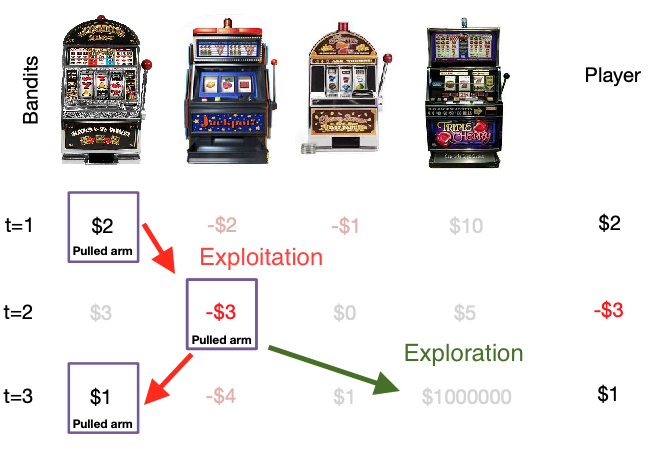
\includegraphics[width=0.8\textwidth]{images/bandits_t_3.png}
    \caption{Illustration of the Exploration-Exploitation trade-off.}
    \label{fig:explore-exploit}
\end{figure}

Since there is only a partial observability in the MAB scenario, we only know about the performance of a subset
of the arms in hindsight. Thus we have two choices:
\begin{enumerate}
    \item \textbf{Exploitation}: Player picks the arms that they know have performed well in the past.
    \item \textbf{Exploration}: Player tries picking up new arms for which they have zero evidence.
\end{enumerate}
Figure \ref{fig:explore-exploit} illustrates this point. The player only follows the exploitation strategy and
misses out on a high reward. If the player had followed a \textit{balanced} strategy that allowed for a
\textit{trade-off} between exploration and exploitation, then it might have gotten a larger reward.

A general strategy to avoid this situation is to design algorithms that transition from exploring to exploiting.
Next, we look at one such strategy in a \textit{stochastic} environment, where each arm has a static reward
distribution so that each pull gives a sample from the underlying static distribution. This is precisely the
notion of a \textit{stochastic bandit} presented in \cite{chernoff1959sequential}.

\subsubsection{Explore-exploit algorithm}
Assuming a stochastic bandit, how should the player pull the arms if they have only $T$ rounds? The
Explore-Exploit algorithm aims at answering this question. At a high-level, the algorithm proceeds in two
phases:
\begin{enumerate}
    \item \textbf{Explore Phase}: Pull each arm $M$ times to estimate the mean reward.
    \item \textbf{Exploit Phase}: Keep pulling the arm with the highest expected mean reward until $T$.
\end{enumerate}

Note that there is an assumption here that the total number of trials $T$ is greater than or equal to the product
of the number of arms and $M$.

More formally, let $a_k \in \mathcal{A}$ denote the action for a particular arm and the cardinality of the
set $|\mathcal{A}| = K$ represent the total number of arms. The reward received at time $t$ is denoted by
$r^{(t)}$, the number of exploration steps (per action) by $M$, and the estimated average reward of action
$k$ by $\hat{\mu}_k$. The algorithm is given by:

\begin{algorithm}[H]
\caption{Explore-Exploit}
\label{algo:explore-exploit}
\begin{algorithmic}[1]
\FOR{$k=1 \rightarrow K$}
\FOR{$m=1 \rightarrow M$}
\STATE $a = k$
\STATE Receive($r$)
\STATE $\hat{\mu}_k = \hat{\mu}_k + \frac{r}{M}$
\ENDFOR
\ENDFOR
\FOR{$t = KM \rightarrow T$}
\STATE $a^{(t)} = \arg \max_{k'} \hat{\mu}_{k'}$
\STATE Receive($r^{(t)}$)
\ENDFOR
\end{algorithmic}
\end{algorithm}

Lines 1 to 7 show the exploration phase where each arm $k$ is tried for a total of $M$ times to estimate the
mean reward of the underlying static reward distribution for each arm. Afterwards, lines 8 to 11 show the
exploitation phase which continues after $KM$ timesteps that the exploration phase took until the end at $T$.
Next, we look at the regret bound for this algorithm.

\subsubsection{Regret Bound for Explore-Exploit}
The regret bound for the Explore-Exploit algorithm is given by $O(K^{1/3} T^{2/3})$. The derivation of this bound
requires us to know about the Hoeffding's Inequality \cite{hoeffding1994probability}.

\theorem{\normalfont \textbf{Hoeffding's Inequality} Consider a one-dimension distribution $\nu$ with expectation
$\mu$, where any sample $r \sim \nu$ is bounded such that $r \in [0, 1]$. Given $T$ i.i.d samples, $\{ r^{(t)} \}_{t=1}^T$, we have that for any $\epsilon$: $$p \left( \left| \sum_{t=1}^T \frac{r^{(t)}}{T} - \mu \right| \geq \epsilon \right) \leq 2 e^{-2T\epsilon^2}$$ }

\normalfont
Intuitively, this inequality means that the estimate of the mean gets better with the more samples are available.

% Bandits is exhaustive but Contextual is not why?

%\section*{References}
%Include your references here. Please cite any resources you found useful.	
%Populate the refs.bib file or list your references manually. Be consistent in formatting!
{
\bibliography{refs}
\bibliographystyle{abbrv}
}

%\section{Appendix}
%This section provides any relevant background material that was not covered in the lectures, but was found to be useful for understanding the material. 
%For example, derivations, theory underlying techniques employed, etc. 

%Additionally, this section can summarizes applications or extensions of these techniques found in the literature. 

\end{document} % Done!


